\chapter{Universal Gravitation}
\label{chapter:gravity}


  
\section{Law of Universal Gravitation}
\begin{figure}[ht]
  \centering
  \begin{tikzpicture}[scale=.65]
    \draw[vector,red] (0,0)--(2,0) node[right]{$\bm F_g$};
    \draw[vector,blue] (8,0)--(6,0) node[left]{$\bm F_g$};
    \shade[ball color=red] circle (.7) node[white]{$m_1$};
    \shade[ball color=blue] (8,0) circle (1)  node[white]{$m_2$};
    \draw[dashed] (0,0)--(0,-1.5);
    \draw[dashed] (8,0)--(8,-1.5);
    \draw[axes] (0,-1.3)--(8,-1.3) node[midway,below]{$\bm r_{12}$};
  \end{tikzpicture}
  \caption{Gravitational attraction between two point masses.}
  \label{fig:grav-force}
\end{figure}
In classical mechanics, \textbf{gravity} is a mutually attractive force
between massive objects (shown in Fig.~\ref{fig:grav-force}). The magnitude of
the gravitational force is given by the \textbf{law of universal
  gravitation}\footnote{We now know that the ``law'' of ``universal''
gravitation is neither a law nor is it universal. The law does not apply for
extremely massive objects like black holes and neutron stars, and must be
replaced with general relativity. For extremely small masses, like electrons and
protons, it is not know whether the law applies. We also know that in general
relativity, gravitation is not an actual force, but the rather, the result of
curvature in spacetime.}:
\begin{equation}
  \boxed{
    F_g=\frac{Gm_1m_2}{r^2}
  }
  \label{eq:universal-grav}
\end{equation}
where $G=\SI{6.674e-11}{\newton.\metre\squared\per\kilo\gram\squared}$ is the
\textbf{universal gravitational constant}, $r$ is the distance between the
masses. In this equation, $m_1$ and $m_2$ are \emph{point masses} that do not
occupy any space. By the third law of motion: If $m_1$ exerts a gravitational
force $\bm F_{12}$ on $m_2$, then $m_2$ likewise also exerts a reaction force of
$\bm F_{21}=-\bm F_{12}$ on $m_1$. The two forces are equal in magnitude and
opposite in direction, hence the attraction is \emph{mutual}.

\fcolorbox{black}{magenta!10}{
  \small
  \begin{minipage}{.97\linewidth}
    \textbf{Common Question: What happens when $r=0$?} It is worth pointing out
    that no point masses actually exist, and that even an electron must have a
    definite size. Therefore the situation for $r=0$ will never arise; $F_g$ can
    never reach infinite. From a practical point of view, whether a mass can be
    treated as a point mass is a matter of \emph{scale}. For example, at the
    scale of the solar system, the sun and all the planets, moons, comets can
    all be considered as point masses, but at the surface of an
    irregularly-shaped asteroid, the point mass model would be inaccurate.
  \end{minipage}
}

For a mass subjected to the influence of multiple discrete point masses $m_i$
(Fig.~\ref{fig:multiple-masses}),
\begin{figure}[ht]
  \centering
  \begin{tikzpicture}[scale=.4]
    \shade[ball color=red] circle (.7) node[white]{$M$};

    \draw[vector,blue,rotate=45] (.7,0)--(2.5,0) node[right]{$\bm F_1$};
    \shade[ball color=blue] (5,5) circle (.8) node[white]{$m_1$};

    \draw[vector,green,rotate=-45] (-.7,0)--(-2,0) node[left]{$\bm F_2$};
    \shade[ball color=green] (-5,5) circle (.6) node[white]{$m_2$};

    \draw[vector,violet,rotate=45](-.7,0)--(-3.5,0) node[left]{$\bm F_3$};
    \shade[ball color=violet] (-5,-5) circle (1.2) node[white]{$m_3$};

    \draw[vector,magenta,rotate=-45](.7,0)--(2.7,0) node[right]{$\bm F_4$};
    \shade[ball color=magenta] (5,-5) circle (.8) node[white]{$m_4$};
  \end{tikzpicture}
  \caption{A mass that is subjected to multiple gravitational forces}
  \label{fig:multiple-masses}
\end{figure}
the total gravitational force that $M$ experiences is the vector sum of all
the forces $\bm F_i$:
\begin{equation}
  \boxed{
    \bm F=\sum_i\bm F_i
    =GM\left[\sum_{i=1}^N\frac{m_i}{r_i^2}\hat{\bm r_i}\right]
  }
\end{equation}
At the limit $N\rightarrow\infty$, the summation becomes an integral, and can
now be used to describe the gravitational force from objects with
\emph{spatial extend} i.e.\ masses that take up space (e.g.\ a continuous
distribution of mass):
\begin{equation}
  \boxed{
    \bm F=\int\dl\bm F=GM\int\frac{\dl m}{r^2}\hat{\bm r}
  }
\end{equation}
Objects that are symmetrically spherical (e.g.\ planets are stars in our
solar system) can be treated as point masses, and integration can be avoided.
However, this is not always the case.



\section{Gravitational Field}
As seen in Chapter~\ref{chapter:dynamics}, we generally describe the
gravitational force acting on a mass $m$ (i.e.\ its weight) as:
\begin{equation*}
  \bm F_g=m\bm g
\end{equation*}
where $\bm g$ is the acceleration due to gravity. This equation is always
correct as long as we have the correct magnitude and direction of $\bm g$.
But in light of our new knowledge of the law of universal gravitation in
Eq.~\ref{eq:universal-grav}, to find the gravitational force on $m_2$ in a
two-mass system, we can group the variables in the law of universal
gravitation to find $\bm g$:
\begin{equation*}
  F_g
  =\underbrace{\left[\frac{Gm_1}{r^2}\right]}_{=g}m_2
  =m_2 g
\end{equation*}
The vector field function $g$ is known as the \textbf{acceleration due
  to gravity}, and \textbf{gravitational field}. The gravitational field
$\bm g$ generated by point mass $m$ is a function of the the source mass $m_s$,
and the distance $r$ from it. It shows how it influences the gravitational
forces on other masses:
\begin{equation}
  \boxed{
    \bm g(m_s,\bm r)=-\frac{Gm_s}{r^2}\hat{\bm r}
  }
\end{equation}
The direction of the gravitational field is the inward radial direction
$-\hat{\bm r}$, i.e.\ the direction of $\bm g$ points towards the source mass.

On/near the surface of Earth, we can substitute the mass and radius of Earth
\begin{align*}
  m_1&=m_E=\SI{5.972e24}{\kilo\gram}\\
  r&=r_E=\SI{6.371e6}\metre
\end{align*}
to obtain the commonly-known value of
\begin{align*}
  g &\approx\SI{9.81}{\metre\per\second\squared}\\
  g &\approx\SI{9.81}{\newton\per\kilo\gram}
\end{align*}
both units are equivalent.

When multiple discrete point masses are present, the total gravitational field
at any position $\bm r$ is the vector sum of all the fields $\bm g_i$:
\begin{equation}
  \boxed{\bm g
    =\sum_i\bm g_i
    =G\left(\sum_{i=1}^N\frac{m_i}{r_i^2}\hat{\bm r_i}\right)
  }
\end{equation}
At the limit $N\rightarrow\infty$, the summation becomes an integral, and can
now be used to describe the gravitational field generated by objects with
\emph{spatial extend}:
\begin{equation}
  \boxed{
    \bm g
    =\int\dl\bm g
    =G\int\frac{\dl m}{r^2}\hat{\bm r}
  }
\end{equation} 
This integral may be difficult to compute, if the geometry is complicated.

When a mass $m$ is placed inside a gravitational field $\bm g$, it
experiences a gravitational force given by the familiar equation:
  %$\bm g$ itself doesn't \emph{do} anything unless/until another mass $m$
  %enters the field. Then, $m$ experiences a gravitational force $\bm F_g$
  %proportional to $m$ and $\bm g$, regardless of how the field is created:
\begin{equation*}
  \bm F_g=m\bm g
\end{equation*}
%  Note: A point mass is not affected by the gravitational field that itself
%  generates.


\begin{figure}[ht]
  \centering
  \begin{tikzpicture}
    \draw[blue!70!black,mass] circle (.3) node[midway]{$M$};
    \foreach \theta in {0,45,...,359}
    \draw[vector,blue!70!black,rotate=\theta] (2,0)--+(-1,0);
    \foreach \theta in {0,30,...,359}
    \draw[vector,blue!70!black,rotate=\theta] (3,0)--+(-.4,0);
    \node[right,blue!70!black] at (2,0) {$\bm g$};
    \node[
      text width=140,
      draw=blue!70!black,
      fill=blue!5,
      text=blue!70!black] at (5.7,0) {$M$ generates a gravitational field
      that extends from the mass itself over the entire space, with a magnitude
      of

      \vspace{-.07in}
      \begin{displaymath}
        g=\frac{GM}{r^2}
      \end{displaymath}
      $\bm g$ points \emph{towards} the mass that generated it.
      \par
    };

    \begin{scope}[orange,rotate=20]
      \draw[vector] (-3.5,0)--+(1.2,0) node[right=0]{$\bm F_g$};
      \draw[thick,fill=orange!5] (-3.5,0) circle (.18) node{$m$};
    \end{scope}
    \node[
      text width=220,
      draw=orange,
      fill=orange!5,
      text=orange] at (-2.7,-3.6){Mass $m$ is inside the gravitational field
      generated by {\color{blue!70!black}$M$}, therefore it experiences a
      gravitational force of
      
      \vspace{-.08in}
      \begin{displaymath}
        \bm F_g=m{\color{blue!70!black}\bm g}
      \end{displaymath}
      The gravitational force is in the same direction as
      {\color{blue!70!black}$\bm g$}\par
    };
    
    \node[text width=160,text=blue!70!black] at (5.3,-3) {The
      gravitational field generated by $M$ does not do anything until there
      is another mass inside the field.\par
    };
  \end{tikzpicture}
\end{figure}


\subsection{Gravitational Field Inside a Spherical Shell}
\begin{figure}[ht]
  \centering
  \begin{tikzpicture}[scale=.45]
    \draw[thick,fill=gray] circle(5) node[above]{$m_1$};
    \draw[thick,fill=black!2] circle(4.9);
    \draw[axes,rotate=30] (0,0)--(4.9,0) node[midway,below]{$R$};
    \draw[mass] (1,-1) circle(.2) node[below]{$m_2$};
  \end{tikzpicture}
\end{figure}
Newton used the \textbf{shell theorem} to show that if a mass $m_2$ is
\emph{inside} a spherical shell of mass $m_1$, the gravitational force that
it experiences is \emph{zero}.
\begin{equation}    
  \boxed{
    \bm F_g=
    \begin{cases}
      \bm 0 & \text{if}\;\;r<R\\
      -Gm_1m_2/r^2\hat{\bm r} & \text{otherwise}
    \end{cases}
  }
\end{equation}
It also means that gravitational field is also \emph{zero} inside the shell.
That $\bm g_\text{inside}=\bm 0$ can be calculated by integrating the fields
created by infinitesimal mass elements $\dl m$ at any point inside the shell,
or use a form of \textbf{Gauss's law} for gravity, similar the equation to
find the electric field inside a charged conducting sphere:
\begin{equation}
  \oint\bm g\cdot\dl\bm A=-4\pi GM_\text{encl}
\end{equation}
Gauss's law is studied in further detail for \emph{electric} fields in
Chapter~\ref{chapter:gauss}\footnote{As a quick reference, Gauss's law for
electricity is stated as:
\begin{equation*}
  \oint_\mathcal{S}\bm E\cdot\dl\bm A=\frac{q_\text{encl}}{\epsilon_0}
\end{equation*}
Since gravitational and electric fields share many similarities, we can adapt
it for gravitational field as well All we have to do is to replace electric
field $\bm E$ with gravitational field $\bm g$, enclosed charge $q_\text{encl}$
with enclosed mass $M_\text{encl}$ and the permittivity of free space
$\epsilon_0$ with $\dfrac1{4\pi G}$.}.

The gravitational field strength inside spherical shell is shown in
Fig.~\ref{fig:spherical-shells}.
\begin{figure}[ht]
  \centering
  \begin{tikzpicture}
    \draw[axes] (0,0)--(0,3) node[above]{$|\bm g|$};
    \draw[axes] (0,0)--(5.5,0) node[right]{$r$};
    \draw[thick,dashed] (1,0)--(1,2) node[pos=0,below]{$R$}--(0,2)
    node[left]{$\dfrac{GM}{R^2}$};
    \draw[function,samples=15,smooth,domain=1:5] plot(\x,{2/\x});
    \draw[function] (0,0)--(1,0);
    \draw[function,fill=black!2] (1,0) circle (.06);
    \fill[red!80!black] (1,2) circle (.06);
  \end{tikzpicture}
  \caption{Gravitational field strength inside and outside a spherical shell
    of radius $R$.}
  \label{fig:spherical-shells}
\end{figure}



\begin{figure}[ht]
  \centering
  \begin{tikzpicture}[scale=.45]
    \draw[thick,fill=gray!50] circle(5);
    \draw[thick,fill=gray!10] (-.2,5) rectangle(.2,-5);
    \draw[mass] (0,1) circle(.15) node[right,black]{$m$};
  \end{tikzpicture}
\end{figure}
Suppose you could drill a hole through the Earth and then jump into it. How
long would it take you to emerge on the other side of the Earth?

To calculate this, we need to know how the gravitational force
changes as you fall through Earth.

\begin{figure}[ht]
  \centering
  \begin{tikzpicture}
    \node at (0,0) {\pic{.3}{../universalGravitation/earth-1200px}};
    \draw (-.18,2.35)--(-.18,-2.35);
    \draw (.18,2.35)--(.18,-2.35);
    \fill[gray,opacity=.8] (-.18,2.35) rectangle (.18,-2.35);
    \draw[very thick,fill=gray,opacity=.3] circle (2.35);
    \draw[dashed,very thick,fill=gray,opacity=.5] circle (1.1);
    \node at (0,1.3) {\pic{.018}{../universalGravitation/falling-person}};
    \draw[axes] (3,1.7)--(.5,1.7) node[pos=0,right]{
      \scriptsize The mass above does not contribute to gravity};
    \draw[axes] (3,.5)--(.5,.5) node[pos=0,right]{
      \scriptsize The mass below contributes to gravity};
  \end{tikzpicture}
  \caption{Dividing into above and below}
\end{figure}

As you fall through Earth, we can separate the part of Earth that is
``above'' you, and the part that is ``below'' you
\begin{itemize}
\item The part that is ``above'' you is like the spherical shell, and does
  not contribute to the gravitational field, and therefore does not exert
  any force
\item The part that is ``below'' you gets smaller as you fall towards the
  centre
\end{itemize}



Assuming that Earth's density is uniform, and neglecting air resistance and
other factors, the value of $g$ as the person falls through Earth ($r<R$) is
given by finding how much mass is still ``below'' the person, $M(r)$:
\begin{equation}
  g(r)=\frac{GM(r)}{r^2}\quad\quad M(r)=\frac43\rho\pi r^3\quad\quad
  \rho=\frac{3M_E}{4\pi r_E^3}
\end{equation}
where $M_E$ is the mass of Earth, $r_E$ is the radius of Earth, $\rho$ is the
(constant) density, and $r$ is the distance from Earth's centre. Then $M(r)$
is the amount of mass ``below'' the person as he/she falls towards the centre.

The gravitational field strength inside this hypothetical Earth is a
linear function of distance $r$ from the centre:
\begin{equation}
  g(r)=\frac{GM_E r}{r_E^3}=\left(\frac r{r_E}\right)g_0
\end{equation}
where $g_0=\SI{9.81}{\newton\per\kilogram}$ is the field strength at Earth's
surface, and $r_E=\SI{6371}{\kilo\metre}$ is Earth's radius. The gravitational
field strength inside and outside a uniform sphere is shown as a function
distance $r$ from the centre of the sphere in Fig.~\ref{fig:g-sphere}.
\begin{figure}[ht]
  \centering
  \begin{tikzpicture}
    \draw[axes] (0,0)--(0,3) node[above]{$|\bm g|$};
    \draw[axes] (0,0)--(5.5,0) node[right]{$r$};
    \draw[thick,dashed] (1,0)--(1,2) node[pos=0,below]{$R$}--(0,2)
    node[left]{$\dfrac{GM}{R^2}$};
    \draw[function,domain=1:5] plot(\x,{2/\x});
    \draw[function] (0,0)--(1,2);
  \end{tikzpicture}
  \caption{Gravitational field strength inside and outside a uniform sphere
    of radius $R$.}
  \label{fig:g-sphere}
\end{figure}
The gravitational field strength is zero at the centre inside the sphere, and
the increases linearly to the surface $r=R$, then drops off as $1/r^2$ outside
the sphere.

The gravitational force is the falling mass times the gravitational field:
\begin{equation}
  F_g(r)=-mg=-\left[\frac{mg_0}{r_E}\right] r
\end{equation}
%The fact that gravitational field scales linearly with $r$ presents an
%interesting situation.
Any mass inside the sphere will experience a force that is proportional to the
distance $r$ from the centre, and in the opposite direction from the
displacement from the centre. This means that gravitational force has the same
form as Hooke's law: it is proportional to displacement from the centre, but in
the opposite direction:
\begin{equation}
  F_g(r)=-kr \quad\text{where}\quad k=\frac{mg_0}{r_E}
\end{equation}
The resulting motion is a simple harmonic motion, with a natural frequency of:
\begin{equation}
  \omega_0=\sqrt{\frac km}=\sqrt{\frac{g_0}{r_E}}
\end{equation}
The traveller will therefore oscillate through Earth with a period of:
\begin{equation}
  T=\frac{2\pi}{\omega_0}=2\pi\sqrt{\frac{r_E}{g_0}}
\end{equation}
For Earth, $T=\SI{5068}\second$. The traveller would pop up on the opposite
side every 42 minutes. Since simple harmonic motion is a projection of a
uniform circular motion, if a satellite is in a circular orbit just above the
surface, and passes overhead just above the traveller as he/she popped up out
of the hole. The period of such an orbit would be the same as oscillating
traveller (Fig.~\ref{fig:withsatellite}).
\begin{figure}[ht]
  \centering
  \begin{tikzpicture}
    \node at (0,0) {\pic{.3}{../universalGravitation/earth-1200px}};
    \fill[gray!50,opacity=.5] (-.18,2.35) rectangle (.18,-2.35);
    \draw[very thick] circle (2.35);
    \draw[dashed,very thick,lightgray] circle (2.55);
    \foreach\theta in {5,50,95,140,185}{
      \draw[vector,red,rotate=\theta] (0,2.55) arc(90:105:2.55);
    }
    \node[rotate=-30] at (0,2.5) {
      \pic{.05}{../universalGravitation/6856-small.png}};
    \node[rotate=-210] at (0,-2.5) {
      \pic{.05}{../universalGravitation/6856-small.png}};

    \draw (-.18,2.35)--(-.18,-2.35);
    \draw (.18,2.35)--(.18,-2.35);

    \node at (0,2.2) {\pic{.02}{../universalGravitation/falling-person}};
    
    \draw[vector] (0,1.8)--(0,1.4);
    \draw[vector] (0,1.3)--(0,.6);
    \draw[vector] (0,.5)--(0,-.5);
    \draw[vector] (0,-.6)--(0,-1.3);
    \draw[vector] (0,-1.4)--(0,-1.9);
    \draw[vector] (0,-2)--(0,-2.3);
  \end{tikzpicture}
  \caption{A satellite travelling just above the surface of Earth has the
    same period of motion as the falling traveller.}
  \label{fig:withsatellite}
\end{figure}


\section{Gravitational Field Lines}
\begin{figure}[ht]
  \centering
  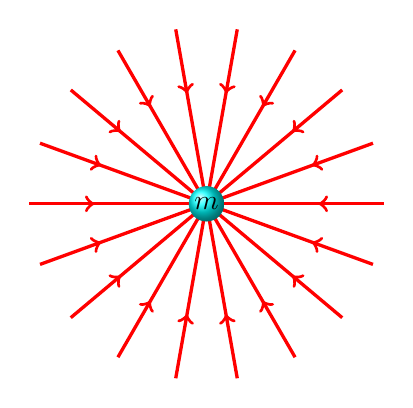
\begin{tikzpicture}[scale=1.5]
    \foreach \x in {0,20,...,359}{
      \begin{scope}[red,very thick,rotate=\x]
        \draw (0,0)--(1,0);
        \draw[<-](.95,0)--(1.5,0);
      \end{scope}
    }
    \shade[ball color=cyan] circle(.15) node{$m$};
  \end{tikzpicture}
  \caption{Gravitational field lines from a point mass.}
  \label{fig:grav-field-lines}
\end{figure}
%\begin{itemize}
%\item The direction of $\bm g$ is towards the centre of the object that
%  created it
%\item Field lines do not tell the intensity (i.e.\ magnitude) of $\bm g$,
%  only the direction
%\end{itemize}
%
%When there are multiple masses, the total gravitational field (dotted line)
%is the vector sum of all the individual fields.
%\begin{center}
%  \includegraphics[width=.4\textwidth]{../universalGravitation/grav-fields}
%\end{center}
%The solid lines are called \textbf{equipotential lines}, where the potential
%energy is constant. Equipotential lines are perpendicular to
%gravitational field lines.







\section{Gravitational Potential Energy}

\textbf{Gravitational potential energy} stored between two masses is obtained
by integrating the work ($W_g$) done by the gravitational force ($\bm F_g$):
\begin{equation*}
  W_g =\int \bm F_g\cdot\dl\bm r
  =-\int_{r_0}^{r_1}\frac{Gm_1m_2}{r^2}\hat{\bm r}\cdot\dl\bm r
  =-Gm_1m_2\int_{r_0}^{r_1}\frac{\dl r}{r^2}=\frac{Gm_1m_2} r\Big|^{r_1}_{r_0}
  =-\Delta U_g
\end{equation*}
where the \textbf{gravitational potential energy} is defined as
\begin{equation} 
  \boxed{U_g=-\frac{Gm_1m_2}r}
  \label{eq:real-Ug}
\end{equation}
$U_g$ is the work required to move two objects from $r=r_0$ to $\infty$. From
this equation, $U_g\leq 0$: $U_g=0$ at $r=\infty$ and \emph{decrease} (i.e.\
becomes ``more negative'') as $r$ decreases\footnote{That $U_g$ is negative
should not bother anyone. Even when we expressed the energy as $U_g=mgh$ in
Chapter~\ref{chapter:energy}, we would often get $U_g<0$ when the object is
below the reference level (where $h=0$). Eq.~\ref{eq:real-Ug} allows us to
generalize all gravitational potential energies}. As we have already seen in
Chapter~\ref{chapter:energy}, the work done by gravity is related to the
gravitational potential energy by:
\begin{equation}
  \boxed{
    W_g=-\Delta U_g
  }
\end{equation}
indicating that gravity is a conservative force with the following properties:

\fcolorbox{black}{yellow!10}{
  \small
  \begin{minipage}{.97\linewidth}
    \begin{itemize}[nosep,leftmargin=12pt]
    \item $(+)$ work by gravity decreases gravitational potential energy
    \item $(-)$ work by gravity increases gravitational potential energy
    \item $W_g$ depends on $r_0$ and $r_1$, but not \emph{how}
      it goes from $r_0\rightarrow r_1$ (path independence)
    \item Only work done by gravity can affect gravitational potential energy
    \end{itemize}
  \end{minipage}
}

that we are familiar with from Chapter~\ref{chapter:energy}.

The fundamental theorem of calculus shows that gravitational force
$\bm F_g$ is the \emph{negative gradient} of the gravitational potential
energy $U_g$. The direction of $\bm F_g$ would therefore always point from
high to low potential energy. For a point mass, we can express this
relationship by:
\begin{equation}
  \bm F_g = -\nabla U_g = -\diffp{U_g}r\hat{\bm r}
\end{equation}
As is the case in Chapter~\ref{chapter:energy}, an object moving along the
direction of $\bm F_g$ is always decreasing in $U_g$, and the direction of
$\bm F_g$ is called the \emph{steepest descent direction}; it is the shortest
path to decrease $U_g$. Objects travelling perpendicular to $\bm F_g$ would
have a constant $U_g$.

Knowing that $\bm F_g$ and $\bm g$ only differ by a constant (mass $m$), we
can also relate gravitational field to potential energy by the gradient
operator:
\begin{equation}
  \bm g=-\nabla V_g=-\diffp{V_g}r\hat{\bm r}
  \quad\text{where}\quad
  V_g=\frac{U_g}m
\end{equation}
%We already know that the direction of $\bm g$ is the same as $\bm F_g$, i.e.
%\begin{itemize}
%\item The direction of $\bm g$ is the shortest path to decrease $U_g$ 
%\item Objects travelling perpendicular to $\bm g$ has constant $U_g$
$V_g$ is called the \textbf{gravitational potential} but it is rarely used.
However, there is a similar concept called the ``electric potential'' when
dealing with electric field, electric force, and electric potential energies
between charged particles, that will be studied in
Chapter~\ref{chapter:electrostatics1}.


\subsection{Gravitational Potential Energy of Multiple Masses}
When there are multiple masses present, the total energy stored between them is
the sum of the energies stored in all the two-mass systems.

\begin{figure}[ht]
  \centering
  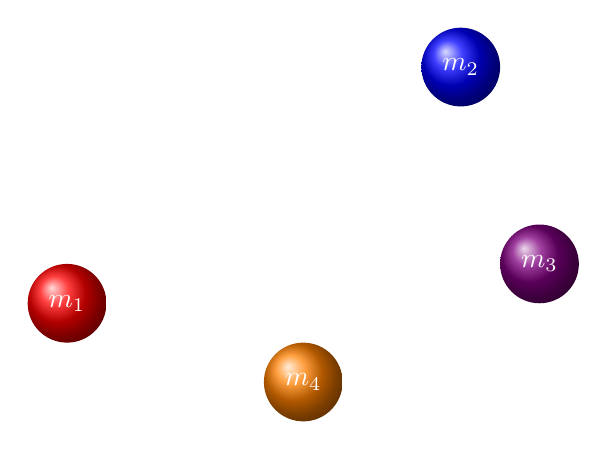
\begin{tikzpicture}
    \shade[ball color=red] circle (.5) node[white]{$m_1$};
    \shade[ball color=blue] (5,3) circle (.5) node[white]{$m_2$};
    \shade[ball color=violet] (6,.5) circle (.5) node[white]{$m_3$};
    \shade[ball color=orange] (3,-1) circle (.5) node[white]{$m_4$};
  \end{tikzpicture}
\end{figure}


\chapter{Orbital Mechanics}
We turn our attention to applying the law of universal gravitation to the
orbital motion of planets and stars in our solar system. To start,
%\section{Properties of Gravitational Force}
two properties of gravity are crucial to understanding of orbital mechanics:
\begin{enumerate}
\item Gravity is a \emph{conservative force}, in that
  \begin{itemize}[nosep]
  \item The total mechanical energy of objects under gravity is constant
  \item Work done by gravity converts gravitational potential energy $U_g$
    into kinetic energy $K$; work against gravity converts $K$ into $U_g$
  \end{itemize}
\item Gravity is a \emph{central force}, in that
  \begin{itemize}[nosep]
  \item Gravitational force $\bm F_g$ is always in the $-\hat{\bm r}$
    direction, i.e.\ $\bm F\times\bm r=\bm 0$
  \item Therefore gravity doesn't generate any torque
  \item And therefore angular momentum $\bm L$ is constant
  \end{itemize}
\end{enumerate}
The above properties are true regardless of the shape of the orbit, and even
for objects that are not in orbit at all (e.g.\ an asteroid slingshotting
around the sun). In \emph{Treatise of the System of the World}, the third book
in \emph{Principia}, Newton presented a thought experiment, shown in
Fig.~\ref{fig:thought-experiment}. A cannonball is shot parallel to the surface
of Earth with some initial velocity $\bm v$.
\begin{figure}[ht]
  \centering
  \begin{subfigure}{.24\textwidth}
    \centering
    \begin{tikzpicture}
      \node at (0,0) {\pic{.8}{../universalGravitation/earth-1200px}};
      \draw[function] ellipse (1 and 1.7);
      \draw[dashed,gray,thick] circle (1.7);
    \end{tikzpicture}
    \caption{The object falls onto the planet after travelling a short distance}
  \end{subfigure}
  \begin{subfigure}{.24\textwidth}
    \centering
    \begin{tikzpicture}
      \node at (0,0) {\pic{.8}{../universalGravitation/earth-1200px}};
      \draw[function] ellipse (1.3 and 1.7);
      \draw[dashed,gray,thick] circle (1.7);
    \end{tikzpicture}
    \caption{The object travels a longer distance but eventually, it still
      falls}
  \end{subfigure}
  \begin{subfigure}{.24\textwidth}
    \centering
    \begin{tikzpicture}
      \node at (0,0) {\pic{.8}{../universalGravitation/earth-1200px}};
      \draw[function,->] (0,1.7) arc (90:-270:1.7);
    \end{tikzpicture}
    \caption{The object stays on a circular path around the planet without
      falling}
    \label{fig:in-orbit}
  \end{subfigure}
  \begin{subfigure}{.24\textwidth}
    \centering
    \begin{tikzpicture}
      \node at (0,0) {\pic{.8}{../universalGravitation/earth-1200px}};
      \draw[dashed,gray,thick] circle (1.7);
      \draw[function,->,domain=0:2.2] plot(\x,{-.3*\x*\x+1.7});
    \end{tikzpicture}
    \caption{The object escapes the gravitational pull of the planet}
    \label{fig:escape-from-orbit}
  \end{subfigure}
  \caption{Newton's thought experiment}
  \label{fig:thought-experiment}
\end{figure}

We want to answer the questions:
\begin{enumerate}
\item How fast does the cannonball have to travel before it goes around Earth
  without falling? (i.e.\ goes into orbit)
\item How fast does the cannonball have to travel before it never comes back?
\end{enumerate}

\section{Orbital Speed}
The example shown in Fig.~\ref{fig:in-orbit} (``fast enough that it doesn't
fall down'') is that of an object moving in circular motion around the planet.
If we assume that a small mass $m$ is in a circular orbit around a much larger
mass $M$, we can further assume that $M$ is stationary. The distance $r$
between the masses is also the orbital radius of that circular motion, and the
centre of $M$ is also the centre of the circula motin. The required centripetal
force is supplied by the gravitational force. Since there are no other forces,
the object moves in uniform circular motion with a constant speed
$v_\text{orbit}$, called the \textbf{orbital speed}, and the velocity vector
$\bm v_\text{orbit}$ is called the \textbf{orbital velocity}. This is shown
graphically in Fig.~\ref{fig:orbital-velocity}.
\begin{figure}[ht]
  \centering
  \begin{tikzpicture}
    \node at (0,0) {\pic{.12}{../universalGravitation/earth-1200px}};
    \draw[function,->] (0,3) arc (90:-270:3);
    \begin{scope}[rotate=50]
      \draw[thick] (0,0)--+(0,-.8);
      \draw[very thick,<->] (0,-.5)--(3,-.5) node[midway,fill=white]{$r$};
      \fill circle (.05) node[above]{$M$};
      \draw[vector,violet] (3,0)--+(0,-2) node[right]{$\bm v_\text{orbit}$};
      \draw[mass] (3,0) circle (.07) node[above]{$m$};
    \end{scope}
  \end{tikzpicture}
  \caption{Object travelling in a circular orbit at the orbital velocity.}
  \label{fig:orbital-velocity}
\end{figure}

Starting with the second law of motion, $\bm F_c=m\bm a_c$, and substituting
the gravitational force $F_g$ into the expression for centripetal force:
\begin{equation}
  F_g=ma_c\quad\longrightarrow\quad \frac{GMm}{r^2}=\frac{mv^2}r
\end{equation}
cancelling the $r$ and $m$ terms on both sides of the equation, we can solve
for the expression for orbital speed, which does not depend on the mass $m$
of the object in orbit:
\begin{equation}
  \boxed{v_\text{orbit}=\sqrt{\frac{GM}r}}
\end{equation}
Note that this equation is only applicable for perfectly circular orbits. Like
all uniform circular motion, the direction of $\bm v_\text{orbit}$ is tangent
to the circular path.

\section{Escape Speed}
The case from Fig.~\ref{fig:escape-from-orbit} is that of an object leaving
orbit, and escaping from the gravitational pull of the planet. For this to
happen, the object must have an minimun velocity such that when all of its
kinetic energy at launch is converted into gravitational potential energy,
the object would be infinitely far away from the planet. This minimum speed
is called the \textbf{escape speed} $\bm v_\text{esc}$.
%An object can leave the surface of Earth at any speed. But when all the
%kinetic energy of that object is converted to gravitational potential energy,
%it will return back to the surface of the earth. There is, however, a
%\emph{minimum} velocity at which the object \emph{would not} fall back to
%Earth.

For this problem, we again assume that the mass of the smaller object ($m$) is
constant, and that gravitational force is the only force acting on $m$. Since
gravitational force is conservative, the calculation for escape speed is a
simple exercise in conservation of energy:
\begin{equation}
    K_\text{launch} + U_\text{launch} = K_\infty + U_\infty
\end{equation}
On the left hand side of the equation, the initial gravitational potential
energy at the surface is:
\begin{equation}
  U_\text{launch}=-\frac{GMm}{r_i}
\end{equation}
where $r_i$ is the initial distance from the centre of the planet/star. This
distance does not have to be at the surface. The kinetic energy at launch is:
\begin{equation}
  K_\text{launch}=\frac12mv_\text{esc}^2
\end{equation}
the speed $v_\text{esc}$ at launch is the escape speed that we are seeking. On
the right hand side of the equation, the final gravitational potential energy
is at $r_f=\infty$, where $U_\infty=0$. At this point, the object has
\emph{escaped} the gravitational pull of the planet/star $M$. At this point, it
no longer matters whether the object is in motion or not, therefore the minimum
required kinetic energy at $r=\infty$ is $K_\infty=0$. Setting the right-hand
side to zero, and equating $K_\text{launch}$ to equal to $-U_\text{launch}$, we
get:
%\item The work against gravity converts kinetic energy into gravitational
%  potential energy.
%\item If you start with \emph{more} kinetic energy than required to do all
%  the work, then the object has
%  planet.
%\end{itemize}
\begin{equation}
  \frac12mv_\text{esc}^2=\frac{GMm}{r_i}
\end{equation}
We can then solve for the escape speed:
\begin{equation}
  \boxed{
    v_\text{esc}=\sqrt{\frac{2GM}{r_i}}
  }
\end{equation}
There is a simple relationship between orbital speed and escape speed:
\begin{equation}
  v_\text{esc}=\sqrt2v_\text{orbit}
\end{equation}

\fcolorbox{black}{yellow!10}{
  \small
  \begin{minipage}{.97\linewidth}
    \textbf{Example:} Determine the escape velocity and energy for a
    \SI{1.60e4}{\kilo\gram} rocket leaving the surface of Earth.
  \end{minipage}
%TL  \uncover<2>{
%TL    \vspace{.5in}Note: The equation for the escape speed is based on the object
%TL    have a \emph{constant} mass, which is \emph{not} the case for a rocket
%TL    going into space.
}

It's important to note that the object can escape from the \emph{surface} or
the planet, or it can escape from \emph{orbit}. In Fig.~\ref{fig:two-escapes},
both objects have the same escape velocity.
\begin{figure}[ht]
  \centering
  \begin{subfigure}{.4\linewidth}
    \centering
    \begin{tikzpicture}[scale=1.8]
      \node at (0,0) {\pic{.15}{../universalGravitation/earth-1200px}};
      \draw[thick] circle (.25) node[below]{$M$};
      \draw[thick,dashed] circle (1);
      \draw[mass] (0,1) circle (.05);
      \draw[mass] (2,0) circle (.05);
      \draw[axes] (0,0)--(0,1) node[midway,right=0]{$r$};
      \draw[axes] (0,1) to[out=0,in=135] (2,0);
    \end{tikzpicture}
  \end{subfigure}
  \begin{subfigure}{.4\linewidth}
    \centering
    \begin{tikzpicture}[scale=1.8]
      \node at (0,0) {\pic{.58}{../universalGravitation/earth-1200px}};
      \draw[thick] circle (1) node[below]{$M$};
      \draw[mass] (0,1) circle (.05);
      \draw[mass] (2,0) circle (.05);
      \draw[axes] (0,0)--(0,1) node[midway,right]{$r$};
      \draw[axes] (0,1) to[out=0,in=135] (2,0);
    \end{tikzpicture}
  \end{subfigure}
  \caption{Escape velocity only depends on $M$ and $r$}
  \label{fig:two-escapes}
\end{figure}
The difference is that the object in orbit (left) already has orbital speed
$v_\text{orbit}$, so escaping from that orbit requires only an additional
speed of
\begin{equation}
  \Delta v=v_\text{esc}-v_\text{orbit}=(\sqrt2-1)v_\text{orbit}
\end{equation}



\section{Orbital Energies}
We can obtain the \textbf{orbital kinetic energy} in a perfectly circular
orbit by using the orbital speed in our expression of kinetic energy:
\begin{equation}
  K_\text{orbit}=\frac12mv_\text{orbit}^2=\frac12m
  \left(\sqrt{\frac{GM}r}\right)^2=\boxed{\frac{GMm}{2r}}
\end{equation}
We already have an expression for gravitational potential energy:
\begin{equation}
    U_g=-\frac{GMm}r=-2K_\text{orbit}
\end{equation}
The \textbf{total orbital energy} is the sum of $K$ and $U_g$:
\begin{equation}
  E_T=K_\text{orbit}+U_g=-\frac{GMm}{2r}=-K_\text{orbit}
\end{equation}


\section{Binary Star Systems}
As always, nothing is as simple as is first seems
\begin{itemize}
\item Most AP Problems will be circular instead of elliptical, but you must
  know the nature of gravitational force (conservative, central)
\item The analysis on the slides shown assumes a small mass $m$ orbiting
  around a large mass $M$. In reality:
  \begin{itemize}
  \item Just as planets experience a gravitational force by the Sun, the Sun
    experiences a gravitational force from the planets
  \item The smaller mass $m$ does not actually orbit about the centre of $M$,
    but rather, the \emph{centre of mass between $M$ and $m$}
  \item Especially important when the two objects orbiting each other has
    similar masses (e.g.\ a binary star system)
  \end{itemize}
\end{itemize}


\fcolorbox{black}{violet!5}{
  \small
  \begin{minipage}{.97\textwidth}
    \textbf{Example: Binary System}
    \begin{center}
      \begin{tikzpicture}[scale=.35]
        \fill circle (.1);
        \draw[dashed] circle (4);
        \draw[dashed] circle (8);
        \shade[ball color=red] (4,0) circle (1) node[white]{$m_1$};
        \shade[ball color=blue] (-8,0) circle (.7) node[white]{$m_2$};
        \draw[vector,blue] (-7.3,0)--(-5.3,0) node[above]{$\bm F_g$};
        \draw[vector,red] (3,0)--(1,0) node[above]{$\bm F_g$};
      \end{tikzpicture}
    \end{center}    
    In a binary star system, two stars orbit around their centre of mass. Both
    have the same period, and the gravitational force provides the centripetal
    force, but this time, the distance to the centre of motion is empty space.
  \end{minipage}
}





\section{Elliptical Orbits}
%What if $v_\text{orbit}<v<v_\text{esc}$? What if $v<v_\text{orbit}$?


As shown in Fig.~\ref{fig:circular-elliptical-parabolic-hyperbolic},
depending on the magnitude of $\bm v$ at $P$:
\begin{figure}[ht]
  \centering
  \begin{tikzpicture}
    \node at (0,0) {\pic{.28}{../universalGravitation/earth-1200px}};
    \draw[vector,red] (0,4) arc (90:-250:4);
    \draw[vector,violet,domain={0:4},dash dot] plot(\x,-.1*\x*\x+4);
    %node[right]{$v_\text{esc}$ (parabola)};
    \draw[very thick,blue,dotted] (0,.5) ellipse (3.2 and 3.5);
    \draw[very thick,orange,dashed] (0,-.5) ellipse (4.2 and 4.5);
    \draw[mass] (0,4) circle (.08) node[above]{$P$};
    \draw[vector] (0,4)--(1.5,4) node[above]{$\bm v$};
    \fill (0,-3) circle (.08) node[below]{$P'$};
    \fill (0,-5) circle (.08) node[below]{$P''$};
    \node[above,blue] at (0,-3) {\scriptsize Elliptical};
    \node[above,magenta] at (0,-4) {\scriptsize Circular};
    \node[above,orange] at (0,-5) {\scriptsize Elliptical};
    \draw[thick,|<->] (0,0)--(0,4) node[pos=.6,right]{$r$};
  \end{tikzpicture}
  \caption{Different orbital paths}
  \label{fig:circular-elliptical-parabolic-hyperbolic}
  %\pic{.6}{../universalGravitation/newton-cannon-orbital-types-Seeds}
\end{figure}
\begin{itemize}
\item{\color{magenta}If the object moves at orbital velocity, i.e.\
  $v=v_\text{orbit}$, it will orbit around the planet in uniform circular
  motion. The path is perfectly circular, and the speed is constant.}
\item{\color{violet}If the object is at escape velocity, $v=v_\text{esc}$, it
  will leave the planet's gravitational pull in a parabolic path.}
\item{\color{green!80!black}If the object is faster than escape velocity, i.e.\
    $v>v_\text{esc}$, it will leave the planet's gravitational pull in a
  hyperbolic path.}
\item{\color{orange} If the object is moving faster than the orbital speed, but
  not faster enough for escape speed, i.e.\ $v_\text{orb}<v<v_\text{esc}$, the
  object would be too fast to maintain a circular path, and therefore gain
  altitude, arriving at point $P'$ on the other side of the planet, which is
  the furthest away from the centre. the resulting path is elliptical.}
\end{itemize}


\section{Kepler's Laws of Planetary Motion}
Johannes Kepler (1571--1630) formulated the \textbf{laws of planetary motion}
between 1609 to 1619, by interpreting planetary motion data from his teacher,
Tycho Brahe. It is an improvement over the heliocentric theory of Nicolaus
Copernicus. Expressed in modern language:
\begin{enumerate}
\item\textbf{Law of ellipses:} The orbit of a planet is an ellipse with the
  Sun at one of the two foci.
\item\textbf{Law of equal areas:} A line segment joining a planet and the Sun
  sweeps out equal areas during equal intervals of time
\item \textbf{Law of periods:} The square of the orbital period of a planet
  is proportional to the cube of the semi-major axis of its orbit.
\end{enumerate}



\subsection{Second Law}

\begin{center}
  \fbox{
    \begin{minipage}{.97\textwidth}
      \textbf{Law of Equal Areas: A line segment joining a planet and the Sun
        sweeps out equal areas during equal intervals of time}
    \end{minipage}
  }
  
  \pic{.4}{../universalGravitation/201532-132212364-3243-planet}
\end{center}
The second law of planetary motion is the easiest to proof, by applying the
conservation of angular momentum $\bm L=m(\bm r\times\bm v)$ (gravity is a
central force).


%\begin{frame}{Kepler's Second Law: Law of Equal Areas}
%  \begin{center}
%    \fbox{
%      \begin{minipage}{.9\textwidth}
%        \textbf{A line segment joining a planet and the Sun sweeps out equal
%          areas during equal intervals of time}
%      \end{minipage}
%    }
%  \end{center}

%    \begin{tikzpicture}[scale=1.3]
%      \fill[gray!45](0,0)--(2,3)--(3,2.8)--cycle;
%      \node at (1.7,2) {$d\bm{A}$};
%      \draw[->,thick](0,0)--(2,3)
%      node[midway,left]{$\bm r$} node[pos=.95,right]{$\alpha$};
%      \draw[->,thick](2,3)--(3,2.8) node[midway,above]{$d\bm r$};
%      \draw[dashed](3,2.8)--(0,0);
%      \fill (0,0) circle (.07) node[right]{\tiny\text{Sun}};
%      \fill (2,3) circle (.035) node[above]{\tiny\text{Planet}};
%    \end{tikzpicture}

%    The infinitesimal area $d\bm{A}$ swept out by an object (such as a planet)
%    as it moves in orbit by an infinitesimal amount $d\bm r$ is given by:
%    
%    \eq{-.4in}{
%      dA=\frac12rdr\sin\alpha
%      \;\rightarrow\;
%      d\bm{A}=\frac12\bm r\times d\bm r
%    }
%
%    \vspace{-.15in}Its time derivative is called the \textbf{areal velocity}:
%      
%    \eq{-.15in}{
%      \frac{d\bm{A}}{dt}
%      =\frac12\bm r\times\frac{d\bm r}{dt}
%      =\frac12\bm r\times\bm{v}
%    }

The rate of change of the area ($\dl A/\dl t$) swept out by a planet (called
the \textbf{areal velocity}) is given by:
\begin{equation}
  \diff At=\frac L{2m}=\text{constant}
\end{equation}

The rate a planet sweeps out the area in orbit is its angular momentum around
the sun divided by twice its mass.



\subsection{First Law}
Proofing Kepler's first law requires some understanding the ellipse. If
the law is true, then orbital motion must agree with the equations of an
ellipse.
%\begin{center}
%  \pic{1.1}{../universalGravitation/elliporb}
%\end{center}
  
%  \begin{itemize}
%  \item $r' + r =2a$
%  \item The area of the ellipse is $A=\pi ab$
%  \item The relationship between $r$ and $\theta$ given by:
%
%    \eq{-.1in}{
%        r=\frac{a(1-e^2)}{1+e\cos\theta}
%        \quad\textnormal{\normalsize where}\quad
%        0\leq e < 1
%      }
%    \item when $e=0$ it's a circle: $a=b=r$
%    \item When $e=1$ it's no longer an ellipse
%    \end{itemize}


Most planets in the solar system have very small eccentricity, so their
orbits are fairly close to being circular, but comets are much more eccentric
%\begin{center}
%  \pic{.65}{../universalGravitation/kep5}
%\end{center}
\begin{table}[ht]
  \centering
  \begin{tabular}{l|l}
    \rowcolor{pink}
    \textbf{Object} & $e$ \\ \hline
    Mercury	& \num{.206} \\
    Venus	& \num{.0068} \\
    Earth	& \num{.0167} \\
    Mars	& \num{.0934} \\
    Jupiter	& \num{.0485} \\
    Saturn	& \num{.0556} \\
    Uranus	& \num{.0472} \\
    Neptune	& \num{.0086} \\
    Pluto	& \num{.25} \\ \hline
    Halley's Comet   & \num{.9671} \\
    Comet Hale-Bopp  & \num{.9951} \\
    Comet Ikeya-Seki & \num{.9999}
  \end{tabular}
\end{table}

As $m$ orbits around $M$, there are two velocity components: \textbf{radial
  velocity} $\bm v_r$ and \textbf{angular velocity} $\bm v_\theta$.
\begin{center}
  \begin{tikzpicture}[scale=.55]
    \def\a{4} % semi-major axis
    \def\b{3.25} % semi-minor axis
    \def\angle{150} % angle
    \draw ellipse ({\a} and {\b});% Draw the ellipse
    \draw ({sqrt(\a*\a-\b*\b)},-2.65)--({sqrt(\a*\a-\b*\b)},2.65);
    \draw (-\a-.2,0)--(\a+.2,0);
    \fill ({sqrt(\a*\a-\b*\b)},0) circle (.1) node[below right]{$M$};
    \begin{scope}[rotate around={\angle:({sqrt(\a*\a-\b*\b)},0)}]
      \draw[vector]({sqrt(\a*\a-\b*\b)},0)--(8.5,0)
      node[pos=.45,below]{$\bm r$}
      node[left]{$\bm v_r$};
      \draw[vector] (7.65,0)--(7.65,.85) node[below]{$\bm v_\theta$};
      \fill (7.65,0) circle (.1) node[above]{$m$};
    \end{scope}
    \draw[axes]({sqrt(\a*\a-\b*\b)+.5},0) arc(0:\angle:.5)
    node[midway,above=0]{$\theta$};
  \end{tikzpicture}
\end{center}

\begin{itemize}
\item $\bm v_\theta$ means a centripetal acceleration toward $M$
\item Changes in $\bm v_r$ (i.e.\ acceleration in the radial direction)
  also means a force along $\hat r$
\item Both components of acceleration are due entirely to gravitational
  force toward $M$
\item Applying second law of motion gives a complicated (at least for
  students new to the concept) ordinary differential equation.
\end{itemize}
A full description for solving the differential equation is
presented in the accompanied handout for anyone interested.



The solution to the ODE is the expression for $r(\theta)$, with eccentricity
$e$ determined by a constant $B$ based on initial condition (how the planet
is formed):
\begin{equation}
    r=\left[\frac{L^2}{GMm^2}\right]\frac1{1+e\cos\theta}
    \quad\text{where}\quad  e=\frac{BL^2}{GMm^2}
\end{equation}

The semi-major axis is the average value between the minimum and maximum
values of $r$:
\begin{equation}
  a=\frac12(r_\text{min} + r_\text{max})
  =\left[\frac{L^2}{GMm^2}\right]\frac1{1-e^2}
\end{equation}
We can rearrange the terms to see that this is the equation for an ellipse.



\subsection{Third Law}

\fbox{
  \begin{minipage}{.97\textwidth}
    \textbf{Law of Periods: The square of the orbital period of a planet
      is proportional to the cube of the semi-major axis of its orbit.}
  \end{minipage}
}

\pic{.45}{../universalGravitation/kep8}



The area swept by the planet through one orbital period is the areal velocity
(constant!) integrated by time, from $t=0$ to $t=T$:
\begin{equation}
  A=\int\dl A=\int_0^T\diff At\dl t=\frac L{2m}\int_0^T\dl t=\frac L{2m}T
\end{equation}
  
But this area is an ellipse, given by the equation based on $a$ (semi-major
axis), $b=a\sqrt{1-e^2}$ (semi-minor axis):
\begin{equation}
  A=\pi ab=\pi a^2\sqrt{1-e^2}
\end{equation}
Equating two equations above and squaring both sides give this expression:
\begin{equation}
  T^2=\frac{m^2}{L^2}4\pi^2a^4(1-e^2)
\end{equation}
But we also (from proving the first law) have:
\begin{equation}
  a(1-e^2)=\frac{L^2}{GMm^2}
\end{equation}
Substituting this expression into the equation for the period, and after
some simple algebra, we end up with this expression:
\begin{equation}
  \boxed{
    T^2=\left[\frac{4\pi^2}{GM}\right] a^3
  }
\end{equation}
